\chapter{Resultados e Discussões}

A Fig. \ref{clusterT1} apresenta à variação das propriedades físicas analisadas por agrupamento de classes de rochas para o poço T$1$. Foi utilizado para tal foi adotado um padrão de cores para cada tipo litológico. 

\begin{figure}[H]
	\centering
	\setlength{\fboxsep}{8pt}
	\setlength{\fboxrule}{0.1pt}
	\fbox{
		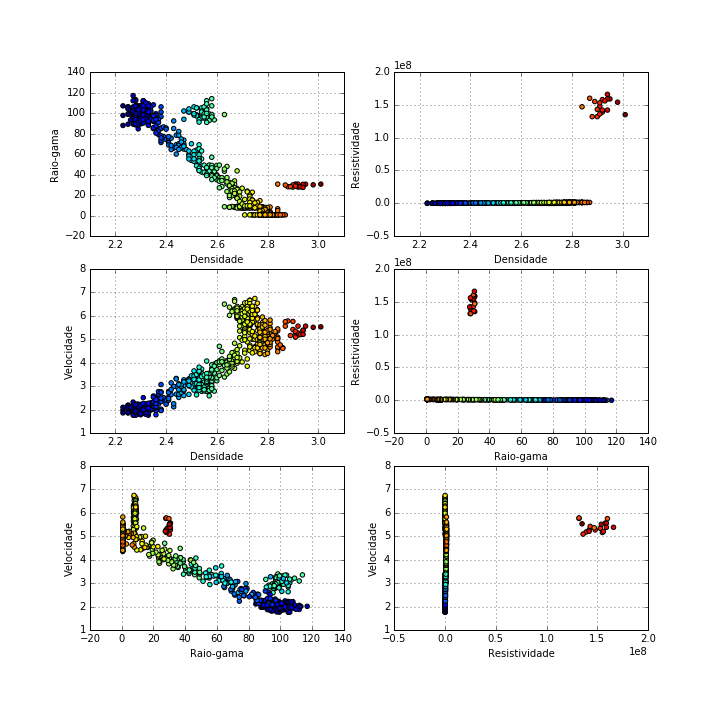
\includegraphics[scale=0.5]{Imagens/cluterpocoT1.png}
	}
	\caption{Agrupamento de dados do poço T1.}
	\label{clusterT1}
\end{figure} 

Em vermelho escuro, se encontra o diabásio, a gradação de cores entre o vermelho claro e o amarelo, se encontra o embasamento, a gradação de cores entre o laranja e o verde claro encontra-se a dolomita, verde claro se encontra o folhelho $2$, a gradação de azul para azul escuro encontra-se o conglomerado, e a gradação que vai do amarelo ao azul são as subclasses de mistura de conglomerado com embasamento de $20\%$, $40\%$, $60\%$ e $80\%$, respectivamente.

É perceptível o notável contraste de variação de resistividade entre a rocha de origem ígnea, em contraste com as propriedades físicas das demais rochas de origem sedimentar e metamórfica. O agrupamento das rochas sedimentares formam um conjunto quase linear próximo a zero.

A Fig. \ref{clusterC1} apresenta à variação das propriedades físicas analisadas por agrupamento de classes de rochas para o poço C$1$.

\begin{figure}[H]
	\centering
	\setlength{\fboxsep}{8pt}
	\setlength{\fboxrule}{0.1pt}
	\fbox{
		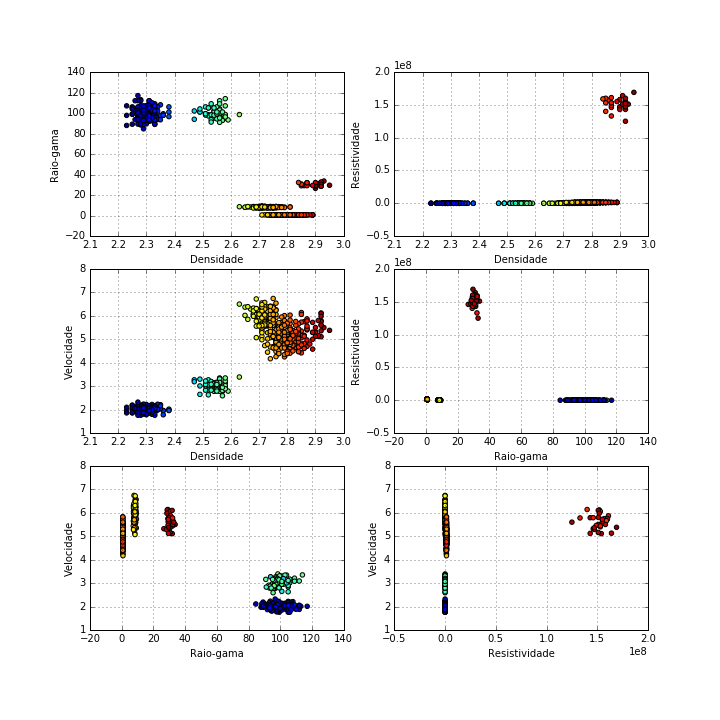
\includegraphics[scale=0.5]{Imagens/cluterpocoC1.png}
	}
	\caption{Agrupamento de dados do poço C1.}
	\label{clusterC1}
\end{figure} 

Neste caso, o agrupamento das classes de rochas é mais evidente, no gráfico de raio-gama por densidade, que evidencia os $5$ litotipos distintamente. E, da mesma maneira, o gráfico de velocidade por densidade.


A Fig. \ref{clusterC2} apresenta à variação das propriedades físicas analisadas por agrupamento de classes de rochas para o poço C$2$. Em destaque, de vermelho, o litotipo diabásio. 

\begin{figure}[H]
	\centering
	\setlength{\fboxsep}{8pt}
	\setlength{\fboxrule}{0.1pt}
	\fbox{
		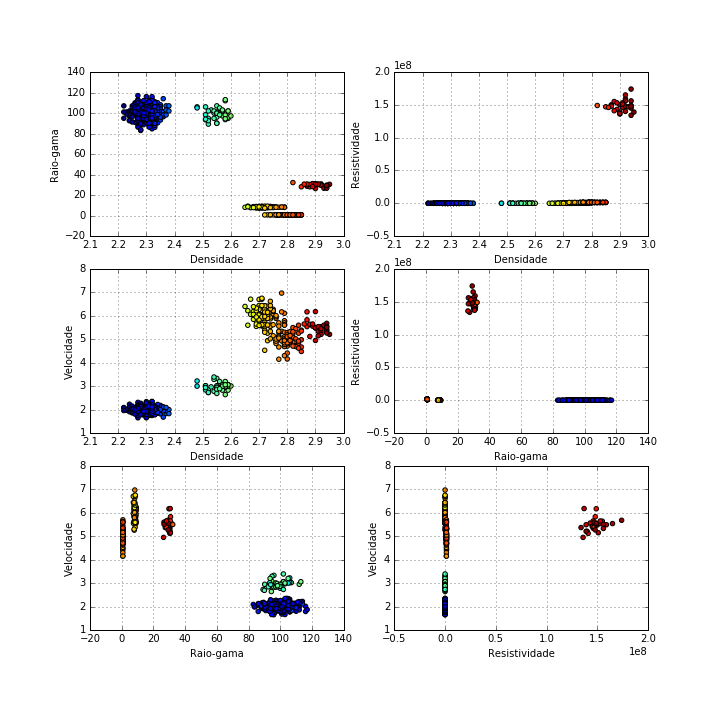
\includegraphics[scale=0.5]{Imagens/cluterpocoC2.png}
	}
	\caption{Agrupamento de dados do poço C2.}
	\label{clusterC2}
\end{figure} 

Na mesma forma, o agrupamento das classes de rochas é mais evidente, no gráfico de raio-gama por densidade, que evidencia os $5$ litotipos distintamente. E, da mesma maneira, o gráfico de velocidade por densidade.

\section{Treinamento}

A etapa de treinamento consiste em um ajuste de pesos dos neurônios da rede. Nesta fase, é identificado o neurônio que tem os valores dos pesos mais parecidos com os parâmetros de entrada da rede.  Por conseguinte, os diversos mapas são obtidos através dos sucessivos ciclos de treinamento ao longo do tempo. A Fig. \ref{SOM}(a), representa a organização da rede com apenas um ciclo de treinamento. Nesta imagem, a rede ainda não é capaz de identificar nenhuma litologia. Ao se aumentar o número de ciclos é perceptível que o ajuste dos pesos cria um conjunto de neurônios vencedores capazes de identificar as classes litológicas. Na quinta iteração, Fig. \ref{SOM}(b), as classes folhelho 2 e dolomita, por exemplo (cores mais azuis) ocupam a maior área do mapa. Já na milésima iteração, Fig. \ref{SOM}(d), a área azul é reduzida dando lugar as cores amarela e verde, que representam as subclasses de conglomerado e embasamento.

\begin{figure}[H]
\centering
\subfigure[ref1][Iteração 1]{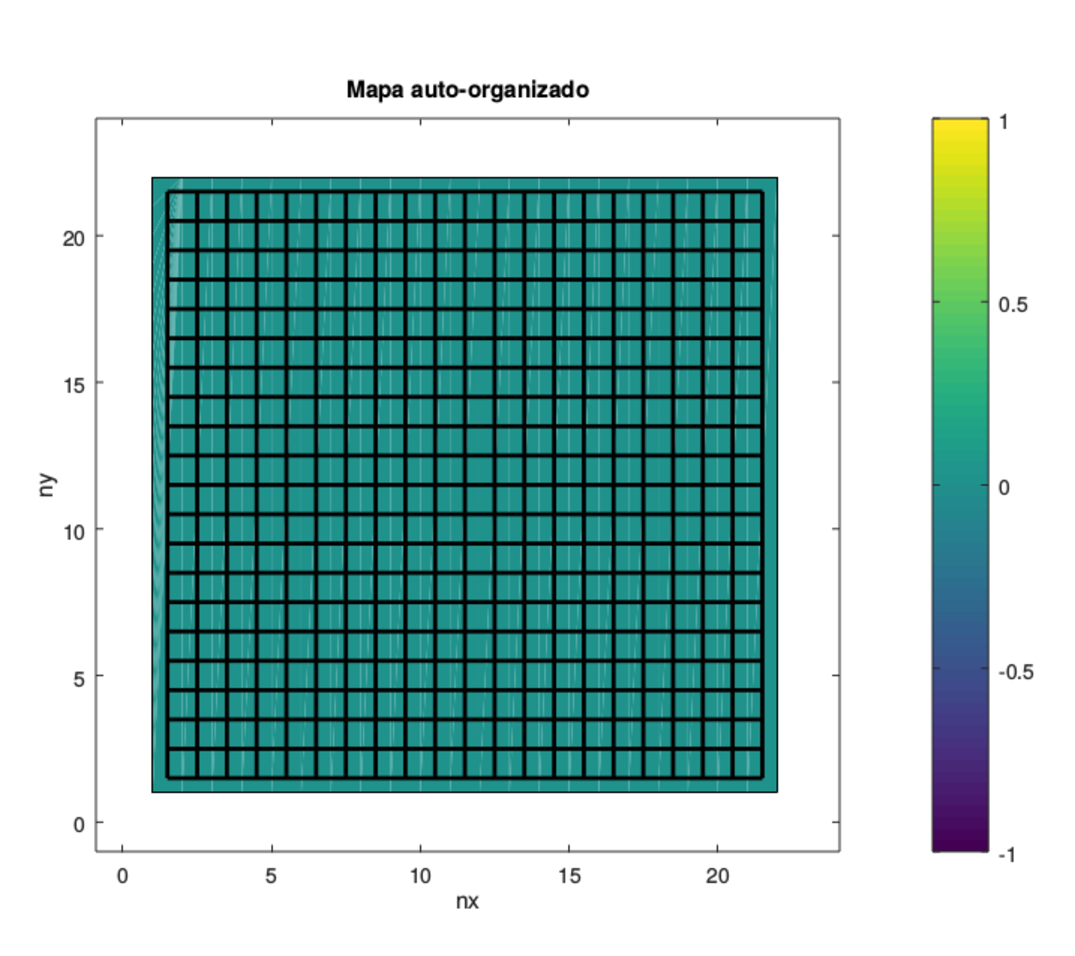
\includegraphics[width=7.0cm]{Imagens/SOM1_2d.pdf}}
\qquad
\subfigure[ref2][Iteração 5]{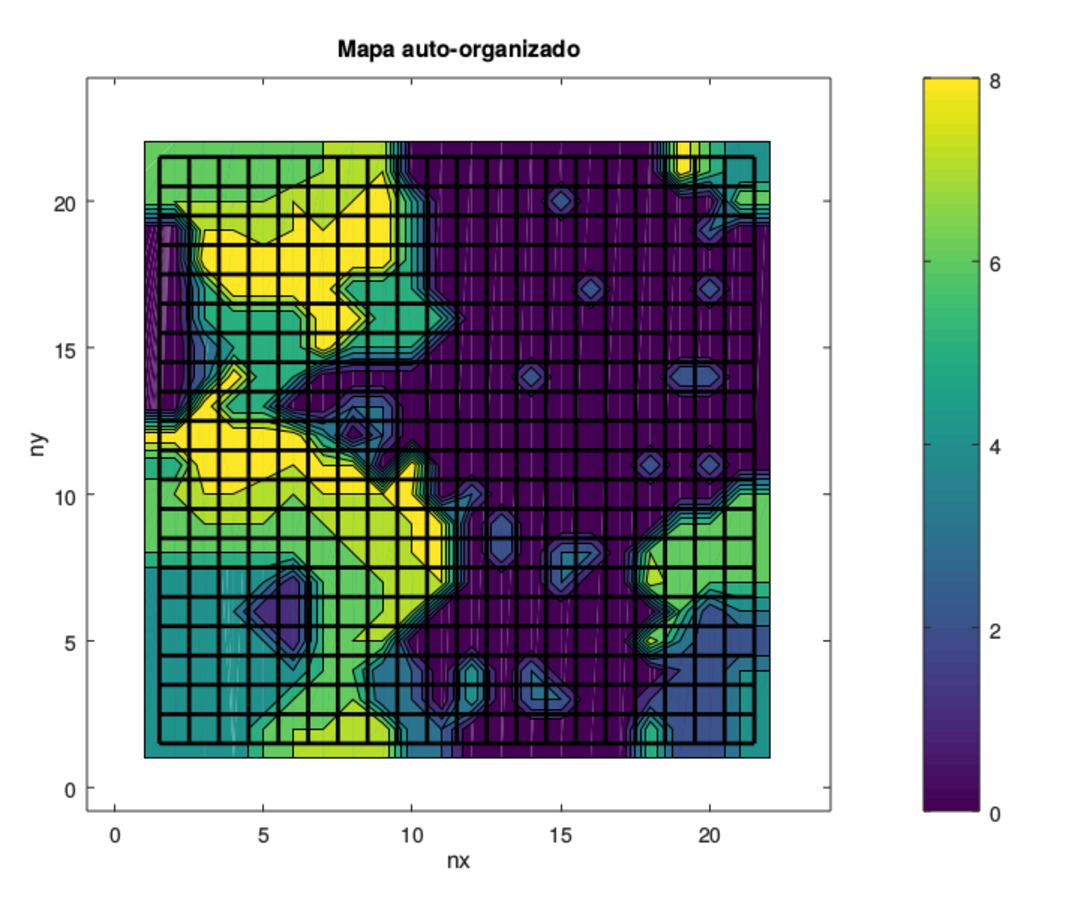
\includegraphics[width=7.0cm]{Imagens/SOM5_2d.pdf}}
\qquad
\subfigure[ref3][Iteração 100]{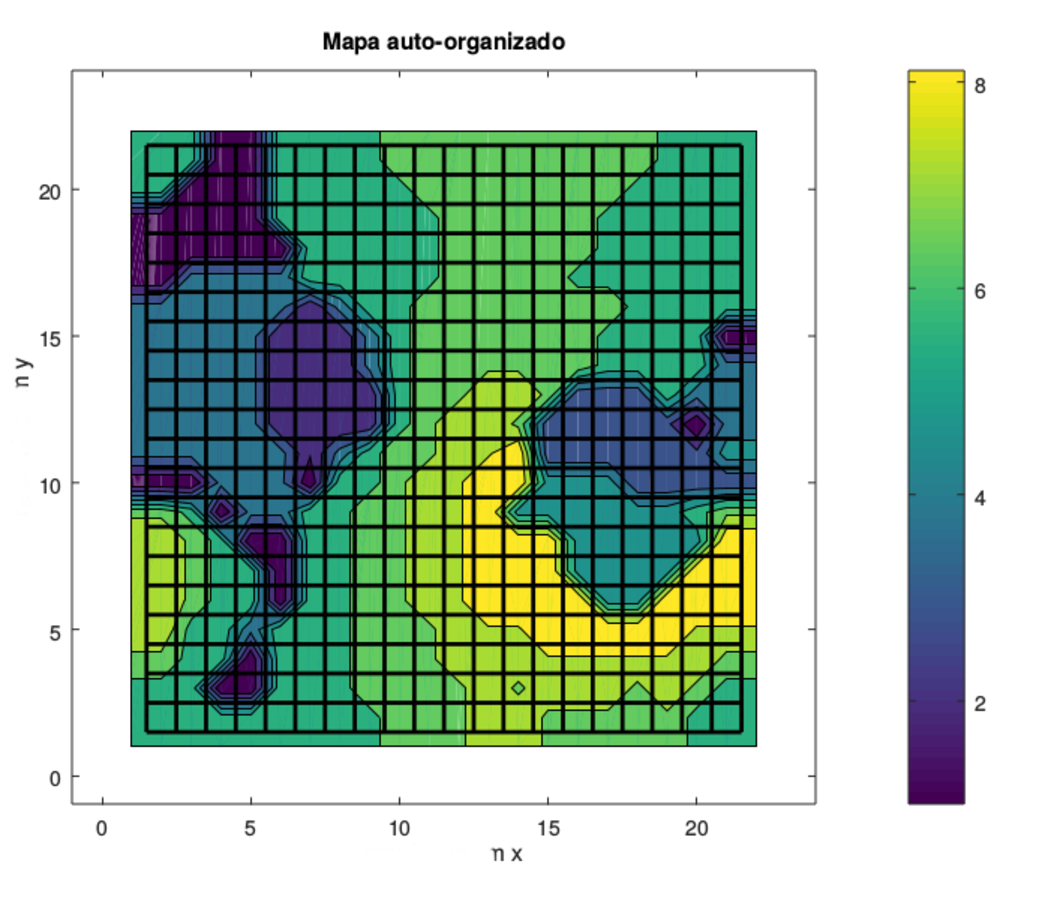
\includegraphics[width=7.0cm]{Imagens/SOM100_2d.pdf}}
\qquad
\subfigure[ref4][Iteração 1000]{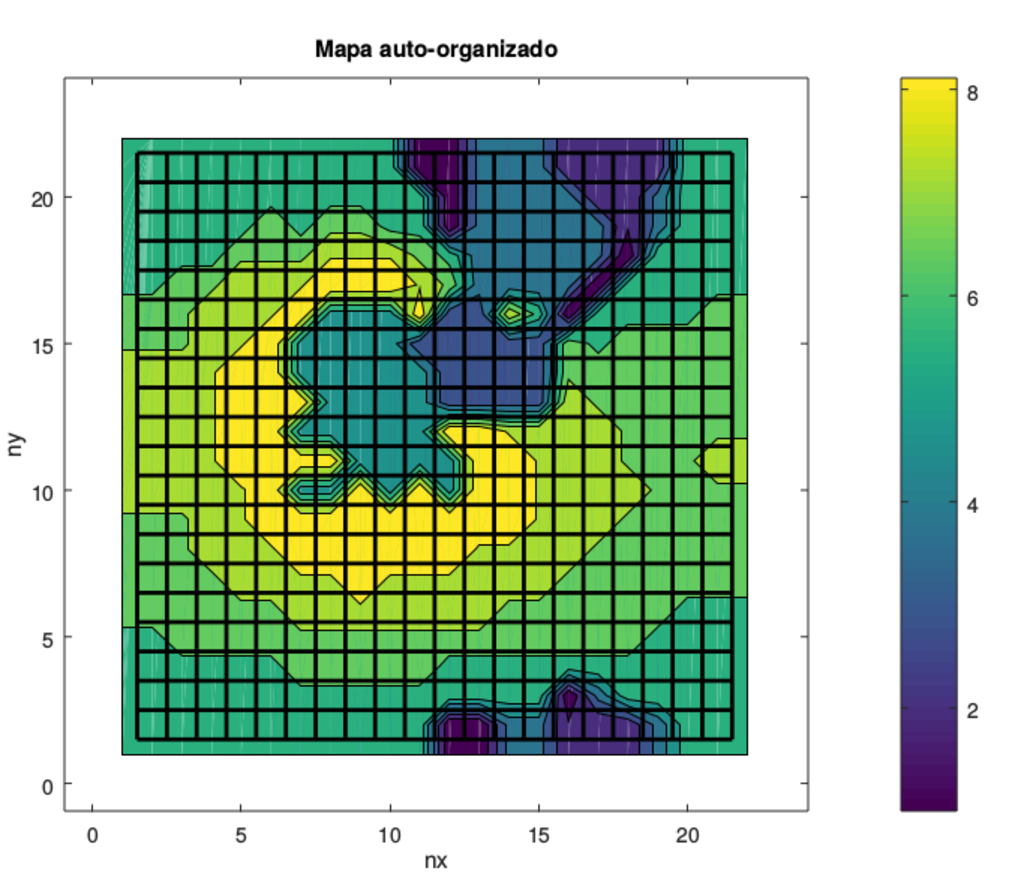
\includegraphics[width=7.0cm]{Imagens/SOM1000_2d.pdf}}
\qquad
\caption{Mapas auto-organizáveis e sua evolução temporal.}
\label{SOM}
\end{figure}

Os mapas da Fig. \ref{SOM} apresentam as zonas do hiperplano especializadas em identificar as classes de rochas. O código numérico $1$ representa folhelho, $2$ dolomita, $3$ diabásio, $4$ conglomerado, $5$ embasamento, $6$ mistura conglomerado/embasamento $80\%$, $7$ mistura conglomerado/embasamento $60\%$, $8$ mistura conglomerado/embasamento $40\%$ e $9$ mistura conglomerado/embasamento $20\%$ . A Tab. \ref{codigos} faz um paralelo entre o código numérico utilizado com \textit{output} da rede e as litologias do modelo.

\begin{table}[H]
	\centering
	\begin{tabular}{c|c}
		
		Litologia                    & Código numérico \\ % Note a separação de col. e a quebra de linhas
		\hline                                                             % para uma linha horizontal
		Folhelho 2                 &  1\\
		Dolomita  		            &  2 \\
		Diabásio    	            &  3 \\
		Conglomerado          &  4 \\
		Conglomerado 80\% &  5  \\
		Conglomerado 60\%&  6 \\
		Conglomerado 40\%&  7\\
		Conglomerado 20\%&  8 \\
		Embasamento          &  9 \\
	 % não é preciso quebrar a última linha
		
	\end{tabular}
	\label{codigos}
	\caption{Tabela de referência para conversão do padrão numérico em litologia.}
\end{table}

A Fig. \ref{convergencia} apresenta o teste de convergência da rede neuronal.

\begin{figure}[H]
	\centering
	\setlength{\fboxsep}{8pt}
	\setlength{\fboxrule}{0.1pt}
	\fbox{
		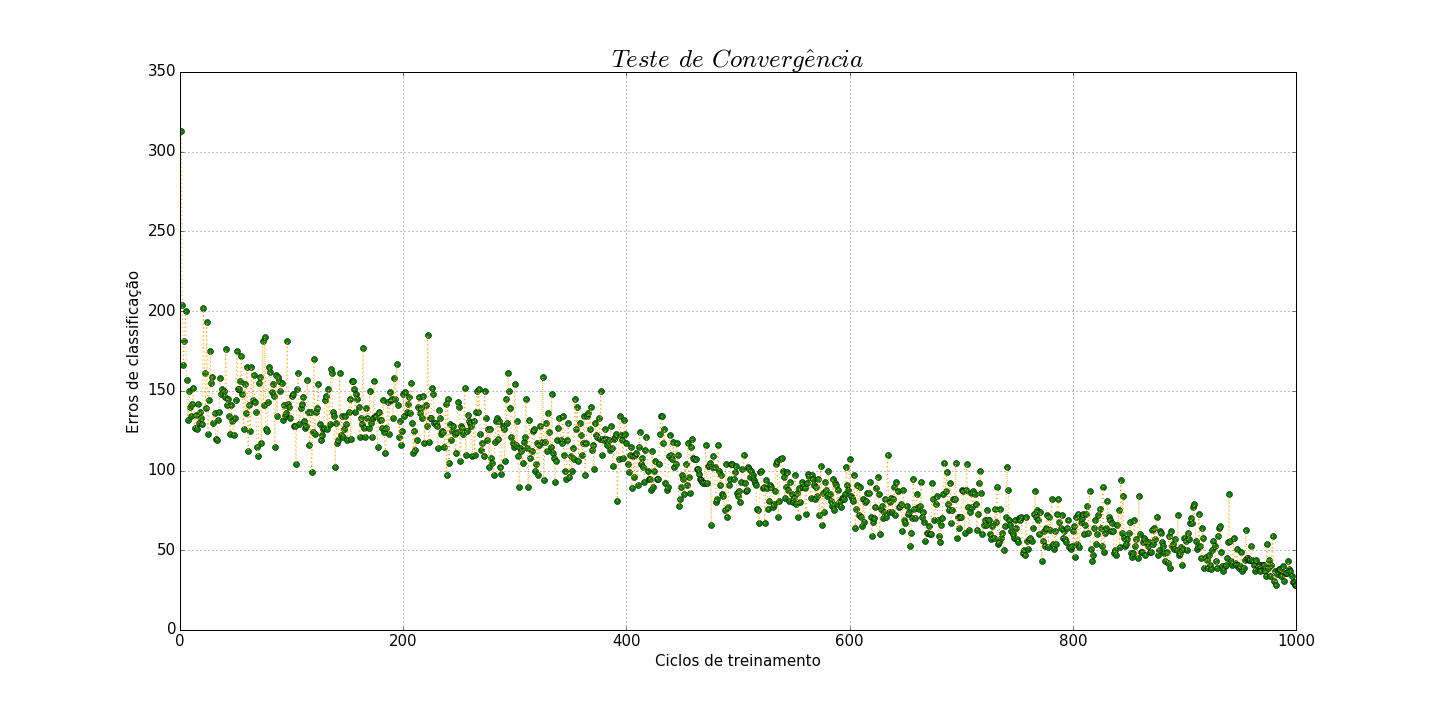
\includegraphics[scale=0.3]{Imagens/conv070917.png}
	}
	\caption{Teste de convergência da rede.}
	\label{convergencia}
\end{figure} 

O teste de convergência é realizado durante a fase de treinamento e mostra que a rede se encontra estabilizada em  $1000$ ciclos de treinamento com $28$ erros de classificação, ou seja, um erro de $4\%$. Isto significa ser inócuo aumentar a iteração afim de diminuir o erro. 



\section{Identificação}

A seguir são apresentados os resultados da etapa de classificação da rede. Nesta fase, dois poços foram utilizados chamados de poços C$1$ e C$2$. O primeiro destes localizado a SW do perfil, Fig. \ref{modelo}, possui $7$km de profundidade. A saída da rede, para o poço C$1$ está localizada ao lado direito da Fig. \ref{Class C1}. Ao lado esquerdo é apresentada o poço original. Abaixo é mostrado uma breve estatística deste processo de identificação 


\begin{figure}[H]
	\centering
	\setlength{\fboxsep}{8pt}
	\setlength{\fboxrule}{0.1pt}
	\fbox{
		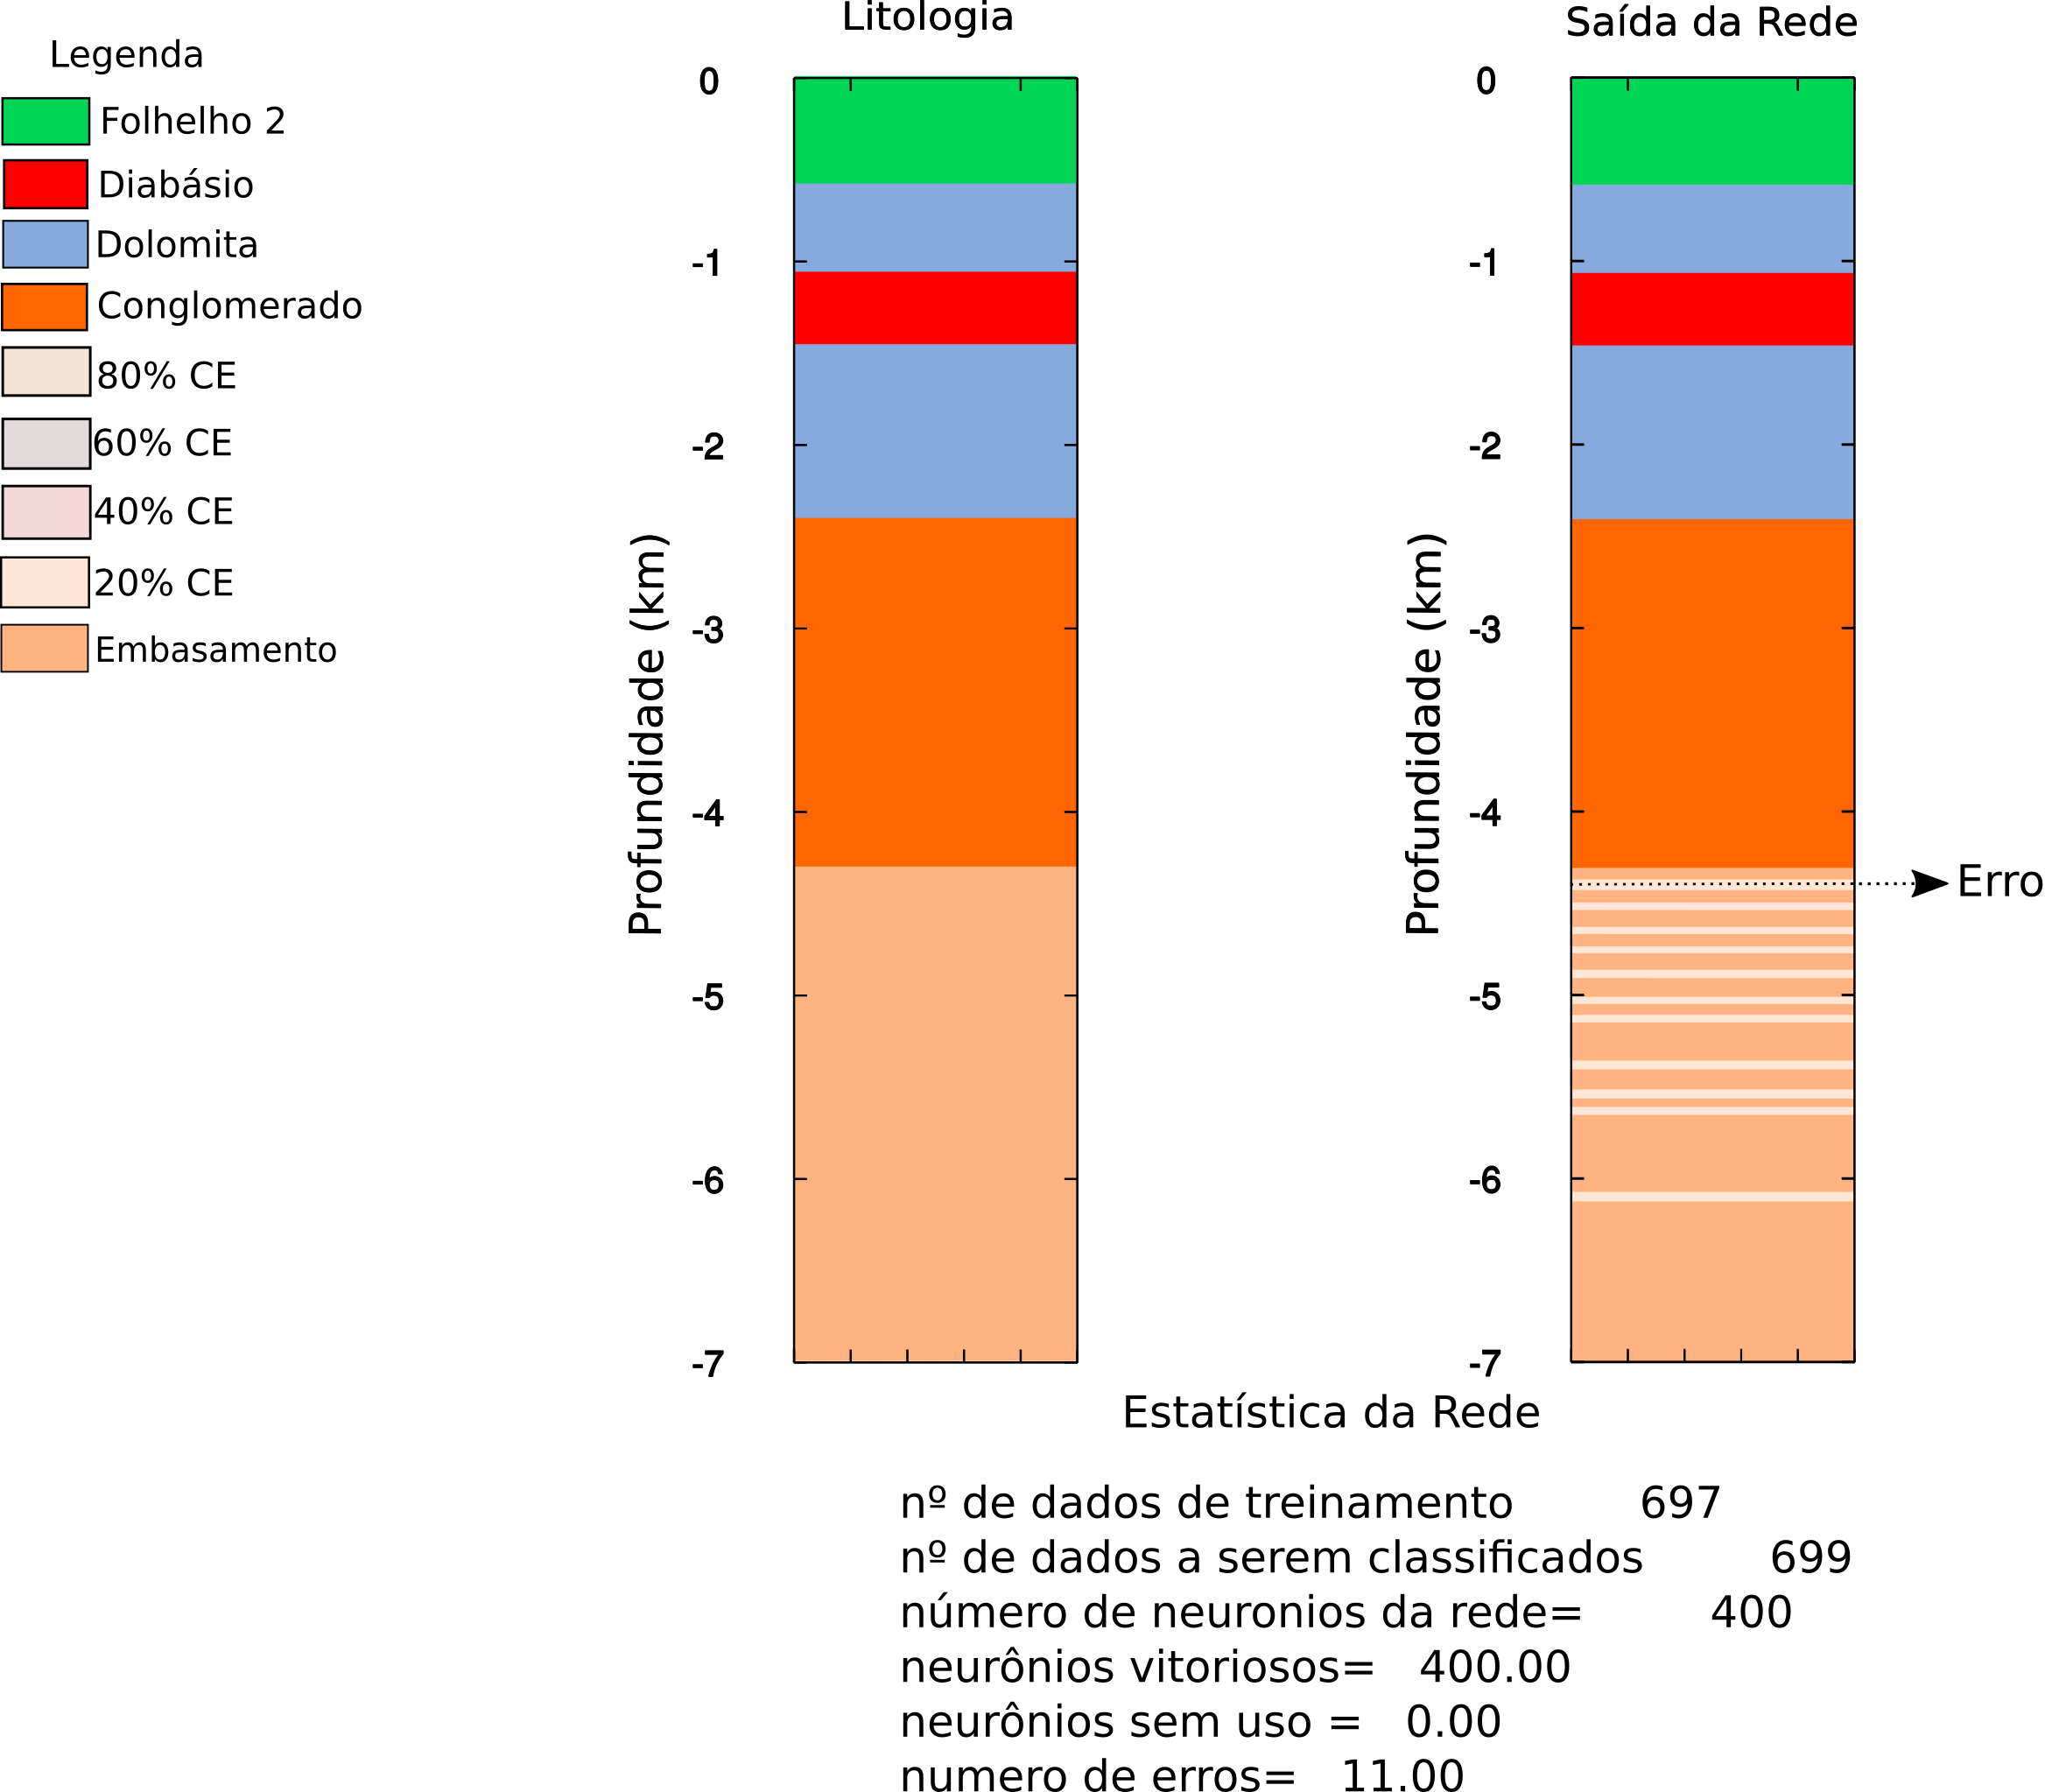
\includegraphics[scale=0.6]{Imagens/IDC1.png}
	}
	\caption{Dado de saída da rede para o poço de classificação C1.}
	\label{Class C1}
\end{figure} 


O processo de identificação foi repetido, contudo, desta vez, para o caso do ao poço C$2$. Este localiza-se mais a NE do perfil, Fig. \ref{modelo}, no topo de um alto estrutural com igual profundidade de $7$ km. A saída da rede, para o poço C$2$ está localizada ao lado direito da Fig. \ref{Class C2}. Ao lado esquerdo é apresentada o poço original. Abaixo é mostrado uma breve estatística do processo de identificação.   


\begin{figure}[H]
	\centering
	\setlength{\fboxsep}{8pt}
	\setlength{\fboxrule}{0.1pt}
	\fbox{
		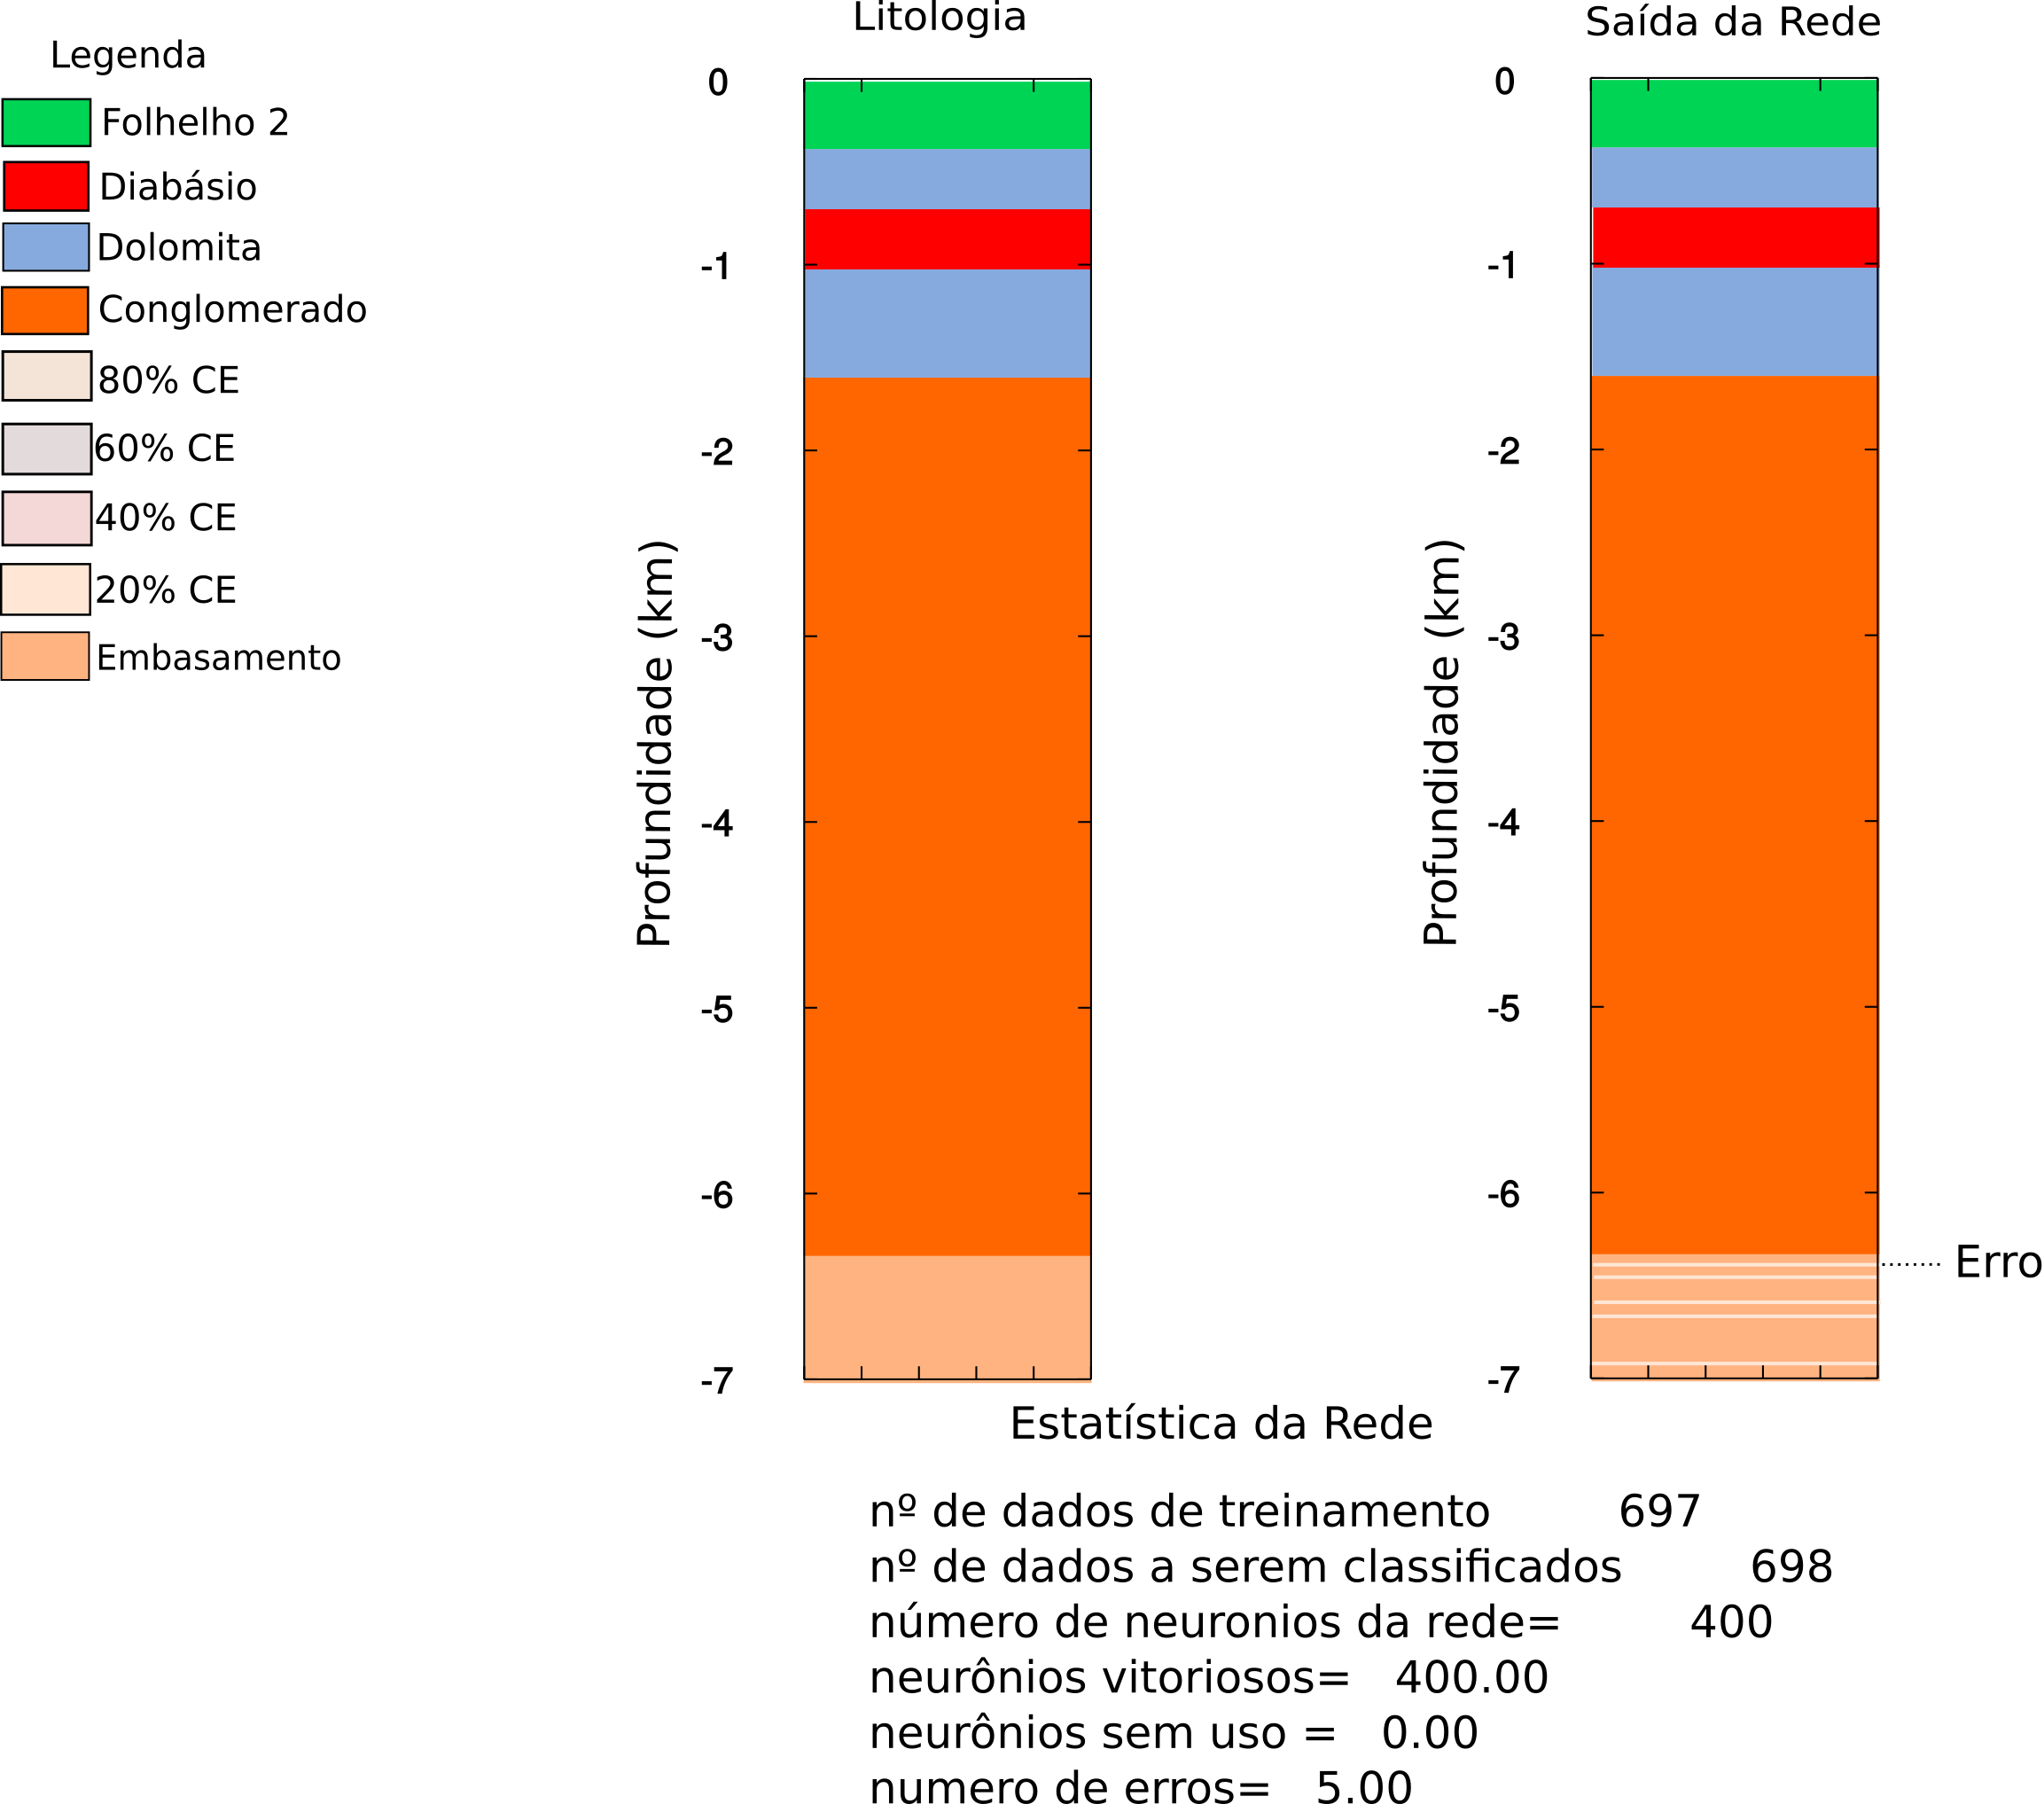
\includegraphics[scale=0.6]{Imagens/IDC2.png}
	}
	\caption{Dado de saída da rede para o poço de classificação C2.}
	\label{Class C2}
\end{figure} 


Em ambos os casos de identificação, o número de neurônios vitoriosos igualou-se ao total de neurônios da rede. Isto indica o máximo de aproveitamento durante os processos, com um tempo de máquina atingindo $25$ segundos.  

